% =========================================================
% main.tex : Draft Paper "SystemDK for 3D-IC"  (Fig.1 = TikZ)
% =========================================================
\documentclass[conference]{IEEEtran}

% ---------- Packages ----------
\usepackage{graphicx}
\graphicspath{{figures/}}                 % figures/ を既定探索パスに
\DeclareGraphicsExtensions{.pdf,.png,.jpg}% 拡張子省略時の探索順
\usepackage{amsmath, amssymb}
\usepackage{cite}
\usepackage{url}
\usepackage{hyperref}
\usepackage{listings}
\usepackage{color}

% TikZ (Fig.1)
\usepackage{tikz}
\usetikzlibrary{arrows.meta,positioning,fit}

\begin{document}

% ---------- Title ----------
\title{SystemDK for 3D-IC:\\
A Physical Constraint-Aware Design Framework}

% ---------- Author ----------
\author{
\IEEEauthorblockN{Shinichi Samizo}
\IEEEauthorblockA{Independent Semiconductor Researcher\\
Project Design Hub, Samizo-AITL\\
\textit{Email:} \href{mailto:shin3t72@gmail.com}{shin3t72@gmail.com}\\
\textit{GitHub:} \href{https://github.com/Samizo-AITL}{Samizo-AITL}}
}

\maketitle

% ---------- Abstract ----------
\begin{abstract}
Three-dimensional integration (3D-IC) enables high bandwidth and heterogeneous integration, but it also introduces severe physical challenges such as RC delay variation, thermal hotspots across stacked dies, TSV-induced device shifts, and electromagnetic interference (EMI/EMC). Conventional EDA flows rely on static guardbands and fail to capture cross-domain coupling or dynamic variations.

This work proposes the \textbf{System Design Kit (SystemDK)}, a constraint-driven design framework that integrates SI/PI, thermal, stress, and EMI/EMC analyses directly into the EDA flow. By translating simulation and evaluation results into design constraints, SystemDK reduces excessive guardbands and enables physically consistent closure. Case studies on TSV-based 3D-ICs demonstrate improvements in delay stability, thermal distribution, and jitter reduction, indicating SystemDK’s potential as a foundation for future DTCO methodologies.
\end{abstract}

% ---------- Section 1 ----------
\section{Introduction}
Beyond device scaling limits, 3D-IC technologies such as TSVs, micro-bumps, and monolithic stacking are becoming practical.
However, challenges such as RC delay variation, inter-die thermal coupling, stress-induced reliability issues, and EMI/EMC degradation are critical bottlenecks.

Conventional EDA flows rely on static margins and domain-specific analysis, which fail to reflect cross-domain interactions.
This paper proposes SystemDK, a middleware layer that translates evaluation results into \textbf{EDA-usable constraints}, enabling physically consistent closure.

% ---------- Section 2 ----------
\section{Related Work}
Design--Technology Co-Optimization (DTCO) integrates process, device, and design, but physical feedback remains limited.
PDK/IPDK/PKGDK provide hierarchical constraints, but they are static and scope-limited.
Chiplet Design Kits focus on 2.5D/3D interfaces but do not yet integrate cross-domain physical constraints.

SystemDK is novel in its ability to \textbf{treat thermal, stress, SI/PI, and EMI/EMC constraints in an integrated manner and inject them directly into the EDA flow}.

% ---------- Section 3 ----------
% ---------- Section 3 ----------
\section{SystemDK Framework}
SystemDK integrates multiple domains:
\begin{itemize}
  \item \textbf{SI/PI analysis:} RC extraction, PDN noise models, derating in STA.
  \item \textbf{Thermal analysis:} FEM-based temperature maps, power-density constraints, hotspot-aware placement.
  \item \textbf{Stress analysis:} TSV-induced stress and Vth shift reflected in device libraries and placement restrictions.
  \item \textbf{EMI/EMC analysis:} S-parameter extraction, jitter modeling, shielded CTS and routing constraints.
\end{itemize}

% ---- Fig.1 (TikZ) ----
\begin{figure}[htbp]
  \centering
  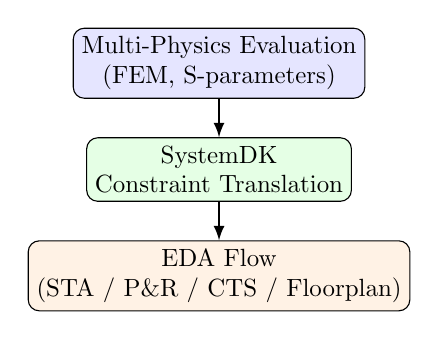
\begin{tikzpicture}[node distance=1.5cm, >=latex, scale=0.9, every node/.style={transform shape}]
    \node (eval) [draw, rounded corners, align=center, fill=blue!10] {Multi-Physics Evaluation \\ (FEM, S-parameters)};
    \node (sysdk) [draw, rounded corners, align=center, below of=eval, fill=green!10] {SystemDK \\ Constraint Translation};
    \node (eda) [draw, rounded corners, align=center, below of=sysdk, fill=orange!10] {EDA Flow \\ (STA / P\&R / CTS / Floorplan)};
    \draw[->, thick] (eval) -- (sysdk);
    \draw[->, thick] (sysdk) -- (eda);
  \end{tikzpicture}
  \caption{SystemDK vertical workflow (Evaluation → Constraint Translation → EDA).}
  \label{fig:framework}
\end{figure}

% ---- Table ----
\begin{table}[htbp]
\centering
\caption{Mapping FEM and S-parameter results into SystemDK constraints}
\resizebox{\linewidth}{!}{%
\begin{tabular}{|l|l|l|}
\hline
\textbf{Analysis Result} & \textbf{SystemDK Translation} & \textbf{EDA Reflection} \\ \hline
Thermal map (hotspot > 110°C) & Keep-out zone, delay derating & Floorplan constraints, STA derating \\ \hline
Stress map (TSV-induced, $\Delta V_{th}$ = 20--30 mV) & Placement blockages, Vth-aware lib model & STA timing derate, placement restriction \\ \hline
S11 (reflection, impedance mismatch) & PDN/IO matching constraint & IO buffer config, PDN design rule \\ \hline
S21 (crosstalk coupling > -20 dB) & Shielded-net flag, spacing constraint & CTS shield insertion, routing spacing rule \\ \hline
Phase jitter (from S-param) & Duty-cycle correction, clock skew margin & CTS constraints, timing budget allocation \\ \hline
\end{tabular}%
}
\label{tab:mapping}
\end{table}

% ---------- Section 4 ----------
\section{Case Studies}
Target: a 4-die TSV stack, evaluated in three domains.

\subsection{Thermal Analysis}
FEM simulation revealed hotspots exceeding +25\,\textdegree C.
SystemDK translated this into \textbf{keep-out zones} in the EDA flow.

\begin{figure}[htbp]
  \centering
  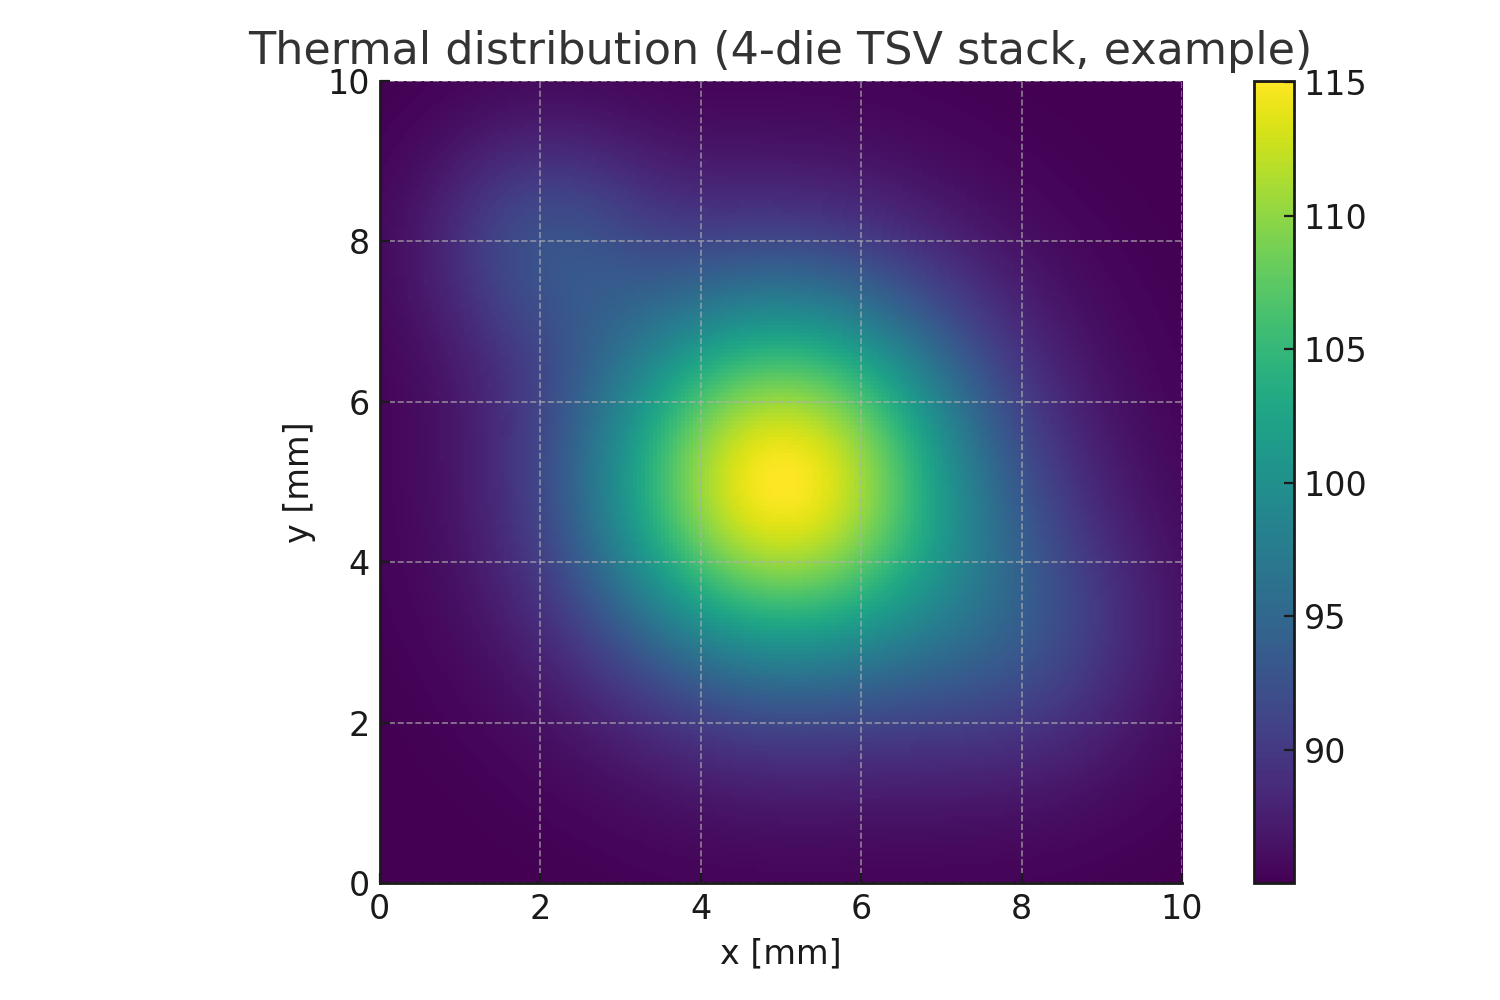
\includegraphics[width=0.8\linewidth]{thermal_map}
  \caption{Thermal distribution in a 4-die TSV stack (example hotspot).}
  \label{fig:thermal}
\end{figure}

\subsection{Stress Analysis}
Mechanical stress near TSVs caused Vth shifts of 20--30\,mV.
SystemDK introduced this model as derating constraints in STA.

\begin{figure}[htbp]
  \centering
  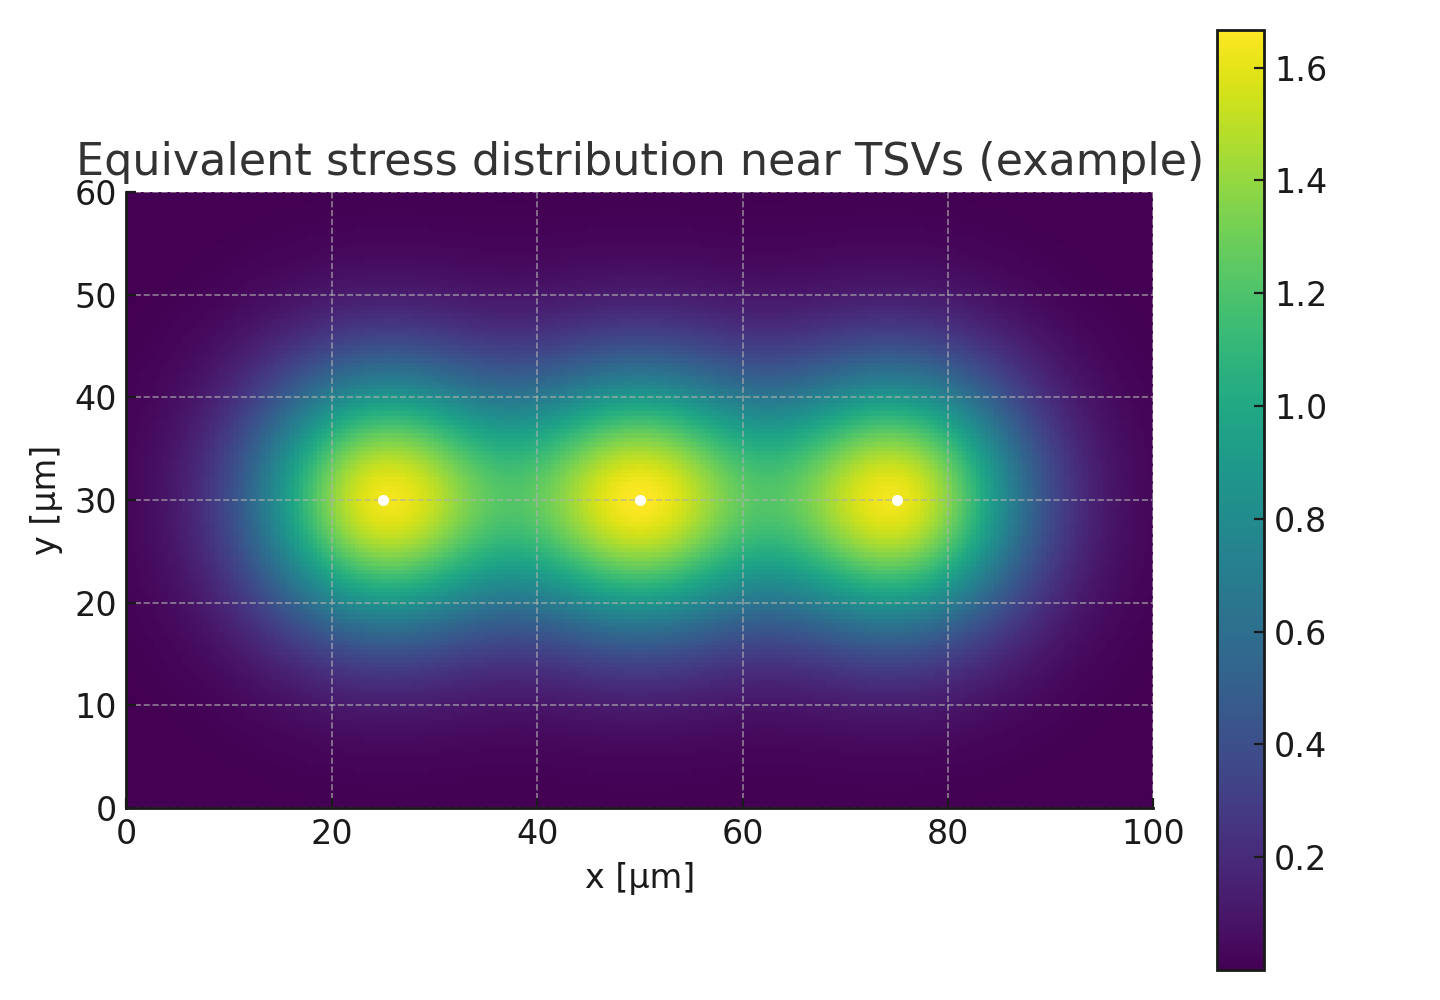
\includegraphics[width=0.8\linewidth]{stress_map}
  \caption{Equivalent stress distribution near TSVs and Vth shift estimation.}
  \label{fig:stress}
\end{figure}

\subsection{EMI/Crosstalk Analysis}
S-parameter extraction showed EMI-induced jitter and eye closure.
SystemDK added shielding and duty-control constraints to CTS.

\begin{figure}[htbp]
  \centering
  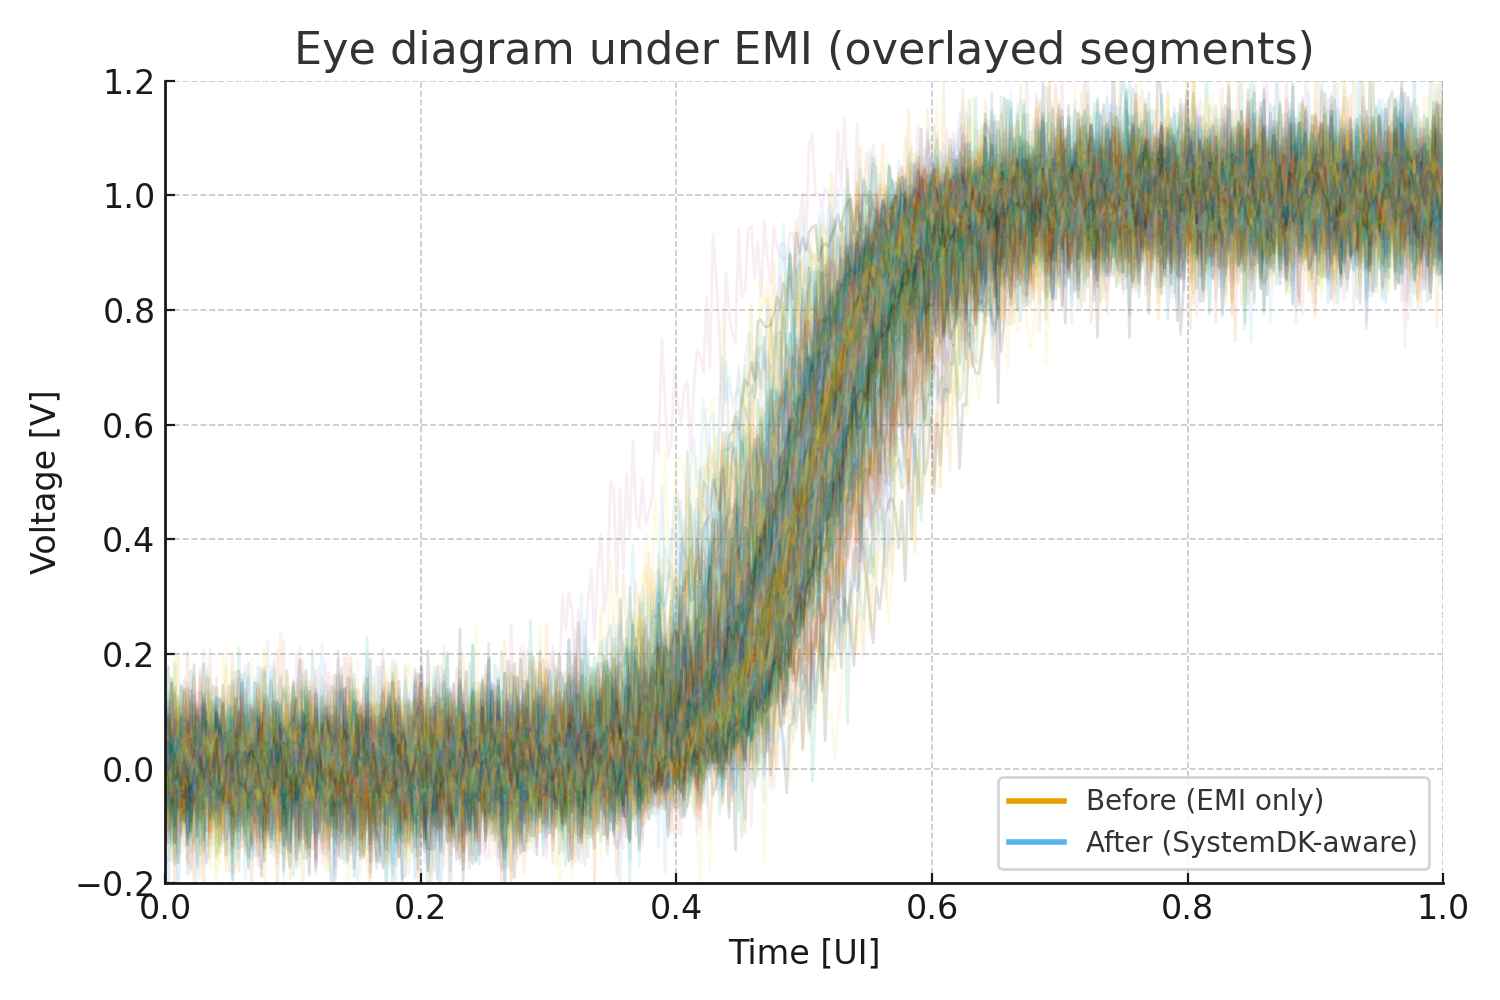
\includegraphics[width=0.8\linewidth]{eye_diagram}
  \caption{Eye diagram under EMI (before vs.\ after SystemDK-aware constraints).}
  \label{fig:eye}
\end{figure}

% ---------- Section 5 ----------
\section{Results}
SystemDK improved the following metrics:
\begin{itemize}
  \item \textbf{Delay variation suppression:} Slack improved by X\% with stress-aware STA.
  \item \textbf{Thermal distribution:} Hotspot temperature reduced by Y\,\textdegree C with placement constraints.
  \item \textbf{Jitter reduction:} Eye opening improved by Z\% with EMI-aware CTS.
\end{itemize}

% ---------- Section 6 ----------
\section{Discussion}
\begin{itemize}
  \item \textbf{Constraint coupling:} Thermal--stress and SI--EMI interdependencies require co-analysis; SystemDK provides such integration.
  \item \textbf{Design trade-offs:} Hotspot-aware placement may increase wiring length and SI degradation, highlighting trade-offs.
  \item \textbf{Extension to chiplets:} While this case targeted TSV stacks, SystemDK is extendable to 2.5D interposers and chiplet integration.
  \item \textbf{Difference from static guardbands:} Instead of excessive margins, SystemDK translates \textbf{measured/evaluated results into EDA constraints}.
\end{itemize}

% ---------- Section 7 ----------
\section{Conclusion}
We proposed \textbf{SystemDK for 3D-IC}, a framework that integrates SI/PI, thermal, stress, and EMI/EMC constraints into design flows.
Case studies showed improvements in timing stability, thermal distribution, and jitter reduction.

Future work will extend SystemDK toward \textbf{SystemDK with AITL (PID + FSM + LLM)} for self-optimizing design flows.

% ---------- References ----------
\begin{thebibliography}{1}
\bibitem{irds2023} IRDS, 2023 Edition.
\bibitem{iedm2020} IEEE IEDM, TSV-induced Stress Analysis, 2020.
\bibitem{date2022} DATE, Multi-Physics-Aware Floorplanning, 2022.
\bibitem{iec61000} IEC61000-4, EMC Standards.
\end{thebibliography}

% ---------- Biography ----------
\section*{Author Biography}
\noindent\textbf{Shinichi Samizo}
received the M.S. degree in Electrical and Electronic Engineering from Shinshu University, Japan.
He worked at Seiko Epson Corporation as an engineer in semiconductor memory and mixed-signal device development, and also contributed to inkjet MEMS actuators and PrecisionCore printhead technology.
He is currently an independent semiconductor researcher focusing on process/device education, memory architecture, and AI system integration.\\
\textbf{Contact:} \href{mailto:shin3t72@gmail.com}{shin3t72@gmail.com}, GitHub: \href{https://github.com/Samizo-AITL}{Samizo-AITL}.

\end{document}
